% defer/rcufundamental.tex

\subsection{RCU Fundamentals}
\label{sec:defer:RCU Fundamentals}
\OriginallyPublished{Section}{sec:defer:RCU Fundamentals}{RCU Fundamentals}{Linux Weekly News}{PaulEMcKenney2007WhatIsRCUFundamentally}

RCU is made up of three fundamental mechanisms, the first being
used for insertion, the second being used for deletion, and the third
being used to allow readers to tolerate concurrent insertions and deletions.
Section~\ref{sec:defer:Publish-Subscribe Mechanism}
describes the publish-subscribe mechanism used for insertion,
Section~\ref{sec:defer:Wait For Pre-Existing RCU Readers}
describes how waiting for pre-existing RCU readers enabled deletion,
and
Section~\ref{sec:defer:Maintain Multiple Versions of Recently Updated Objects}
discusses how maintaining multiple versions of recently updated objects
permits concurrent insertions and deletions.
Finally,
Section~\ref{sec:defer:Summary of RCU Fundamentals}
summarizes RCU fundamentals.

\subsubsection{Publish-Subscribe Mechanism}
\label{sec:defer:Publish-Subscribe Mechanism}

Because RCU readers are not excluded by RCU updaters, an RCU-protected
data structure might change while a reader accesses it.
The accessed data item might be moved, removed, or replaced.
Because the data structure does not ``hold still'' for the reader,
each reader's access can be thought of as subscribing to the current
version of the RCU-protected data item.
For their part, updaters can be thought of as publishing new versions.

% @@@ Merge usage section into "Which to Choose?" and suggest choices.
% @@@ Should "RCU Exercises" move to "RCU Rescues"?

\begin{figure}[tb]
\centering
\resizebox{3in}{!}{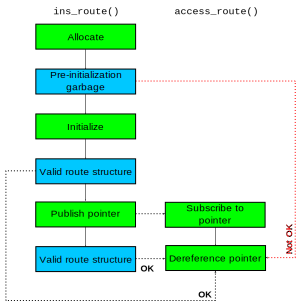
\includegraphics{defer/pubsub}}
\caption{Publication/Subscription Constraints}
\label{fig:defer:Publication/Subscription Constraints}
\end{figure}

Unfortunately, as laid out in
Section~\ref{sec:toolsoftrade:Shared-Variable Shenanigans}
and reiterated in
Section~\ref{sec:defer:Minimal Insertion and Deletion},
it is unwise to use plain accesses for these publication and subscription
operations.
It is instead necessary to inform both the compiler and the CPU
of the need for care, as can be seen from
Figure~\ref{fig:defer:Publication/Subscription Constraints},
which illustrates interactions between concurrent executions of
\co{ins_route()} (and its caller) and \co{read_gptr()} from
Listing~\ref{lst:defer:Insertion and Deletion With Concurrent Readers}.

The \co{ins_route()} column from
Figure~\ref{fig:defer:Publication/Subscription Constraints}
shows \co{ins_route()}'s caller allocating a new \co{route} structure,
which then contains pre-initialization garbage.
The caller then initializes the newly allocated structure, and then
invokes \co{ins_route()} to publish a pointer to the new \co{route}
structure.
Publication does not affect the contents of the structure, which
therefore remain valid after publication.

The \co{access_route()} column from this same figure shows
the pointer being subscribed to and dereferenced.
This dereference operation absolutely must see a valid \co{route}
structure rather than pre-initialization garbage because referencing
garbage could result in memory corruption, crashes, and hangs.
As noted earlier, avoiding such garbage means that the publish and
subscribe operations must inform both the compiler and the CPU of the
need to maintain the needed ordering.

Publication is carried out by \co{rcu_assign_pointer()}, which ensures that
\co{ins_route()}'s callers initialization is ordered before the actual
publication operation's store of the pointer.
In addition, \co{rcu_assign_pointer()} must be atomic in the sense that 
concurrent readers see either the old value of the pointer or the new
value of the pointer, but not some mash-up of these two values.
These requirements are met by the C11 store-release operation,
and in fact in the Linux kernel, \co{rcu_assign_pointer()} is defined
in terms of \co{smp_store_release()}, which is roughly similar to
C11 store-release.

Note that if concurrent updates are required, some sort of synchronization
mechanism will be required to mediate among multiple concurrent
\co{rcu_assign_pointer()} calls on the same pointer.
In the Linux kernel, locking is the mechanism of choice, but pretty
much any synchronization mechanism may be use.
An example of a particularly lightweight synchronization mechanism is
Chapter~\ref{chp:Data Ownership}'s data ownership: If each pointer is
owned by a particular thread, then that thread may execute
\co{rcu_assign_pointer()} on that pointer with no additional
synchronization overhead.

\QuickQuiz{}
	Wouldn't use of data ownership for RCU updaters mean that
	the updates could use exactly the same sequence of instructions
	as would the corresponding single-threaded code?
\QuickQuizAnswer{
	Sometimes, for example, on TSO systems such as x86 or the IBM
	mainframe where a store-release operation emits a single store
	instruction.
	However, weakly ordered systems must also emit a memory barrier
	or perhaps a store-release instruction.
	In addition, removing data requires quite a bit of additional
	work because it is necessary to wait for pre-existing readers
	before freeing the removed data.
} \QuickQuizEnd

Subscription is carried out by \co{rcu_dereference()}, which ensures that
the subscription operation's load from the pointer is ordered before the
dereference.
Similar to \co{rcu_assign_pointer()}, \co{rcu_dereference()} must be
atomic in the sense that the value loaded must be that from a single
store, for example, the compiler must not tear the load.\footnote{
	That is, the compiler must not break the load into multiple
	smaller loads, as described under ``load tearing'' in
	Section~\ref{sec:toolsoftrade:Shared-Variable Shenanigans}.}
Unfortunately, compiler support for \co{rcu_dereference()} is at best
a work in progress~\cite{PaulEMcKennneyConsumeP0190R4,PaulEMcKenney2017markconsumeP0462R1}. @@@ Add JF Bastien's consume paper. @@@
In the meantime, the Linux kernel relies on volatile loads, the details of
the various CPU architectures, coding
restrictions~\cite{PaulEMcKenney2014rcu-dereference},
and, on DEC Alpha~\cite{ALPHA2002}, a memory-barrier instruction.
However, on other architectures, \co{rcu_dereference()} typically
emits a single load instruction, just as would the equivalent single-threaded
code.
The coding restrictions are described in more detail in
Section~\ref{sec:memorder:Address- and Data-Dependency Difficulties},
however, the common case of field selection (\qco{->}) works quite well.
Software that does not require the ultimate in read-side performance
can instead use C11 acquire loads, which provide the needed ordering and
more, albeit at a cost.
It is hoped that lighter-weight compiler support for \co{rcu_dereference()}
will appear sooner rather than later.

In short, use of \co{rcu_assign_pointer()} for publishing pointers and
use of \co{rcu_dereference()} for subscribing to them successfully avoids the
``Not OK'' garbage loads depicted in
Figure~\ref{fig:defer:Publication/Subscription Constraints}.
These two primitives can therefore be used to add new data to linked
structures without disrupting concurrent readers.

\QuickQuiz{}
	But suppose that updaters are adding and removing multiple data
	items from a linked list while a reader is iterating over that
	same list.
	Specifically, suppose that a list initially contains elements
	A, B, and C, and that an updater removes element A and then
	adds a new element D at the end of the list.
	The reader might well see \{A, B, C, D\}, when that sequence of
	elements never actually ever existed!
	In what alternate universe would that qualify as ``not disrupting
	concurrent readers''???
\QuickQuizAnswer{
	In the universe where an iterating reader is only required to
	traverse elements that were present throughout the full duration
	of the iteration.
	In the example, that would be elements B and C.
	Because elements A and D were each present for only part of the
	iteration, the reader is permitted to iterate over them, but not
	obliged to.

	If stronger consistency is required, then higher-cost
	synchronization mechanisms are required, for example, sequence
	locking or reader-writer locking.
	But if stronger consistency is \emph{not} required (and it very often
	is not), then why pay the higher cost?
} \QuickQuizEnd

Adding data to a linked structure without disrupting readers is a good thing,
as are the cases where this can be done with no added read-side cost compared
to single-threaded readers.
However, in most cases it is also necessary to remove data, and this is the
subject of the next section.

@@@

\begin{figure}[tb]
\centering
\resizebox{3in}{!}{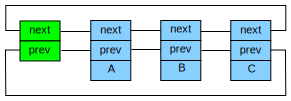
\includegraphics{defer/Linux_list}}
\caption{Linux Circular Linked List}
\label{fig:defer:Linux Circular Linked List}
\end{figure}

\begin{figure}[tb]
\centering
\resizebox{1.8in}{!}{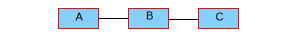
\includegraphics{defer/Linux_list_abbr}}
\caption{Linux Linked List Abbreviated}
\label{fig:defer:Linux Linked List Abbreviated}
\end{figure}

Although \co{rcu_assign_pointer()} and
\co{rcu_dereference()} can in theory be used to construct any
conceivable RCU-protected data structure, in practice it is often better
to use higher-level constructs.
Therefore, the \co{rcu_assign_pointer()} and
\co{rcu_dereference()}
primitives have been embedded in special RCU variants of Linux's
list-manipulation API.
Linux has two variants of doubly linked list, the circular
\co{struct list_head} and the linear
\co{struct hlist_head}/\co{struct hlist_node} pair.
The former is laid out as shown in
Figure~\ref{fig:defer:Linux Circular Linked List},
where the green (leftmost) boxes represent the list header and the blue
(rightmost three) boxes represent the elements in the list.
This notation is cumbersome, and will therefore be abbreviated as shown in
Figure~\ref{fig:defer:Linux Linked List Abbreviated},
which shows only the non-header (blue) elements.

\begin{figure}[tb]
\centering
\resizebox{3in}{!}{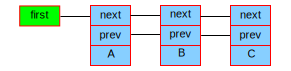
\includegraphics{defer/Linux_hlist}}
\caption{Linux Linear Linked List}
\label{fig:defer:Linux Linear Linked List}
\end{figure}

Linux's other doubly linked list, the hlist,
is a linear list, which means that
it needs only one pointer for the header rather than the two
required for the circular list, as shown in
Figure~\ref{fig:defer:Linux Linear Linked List}.
Thus, use of hlist can halve the memory consumption for the hash-bucket
arrays of large hash tables.
As before, this notation is cumbersome, so hlists will be abbreviated
in the same way lists are, as shown in
Figure~\ref{fig:defer:Linux Linked List Abbreviated}.

@@@

\begin{table*}[tb]
\renewcommand*{\arraystretch}{1.2}
\centering
\footnotesize\OneColumnHSpace{-0.4in}
\begin{tabular}{llll}
\toprule
Category  & Publish	& Retract	& Subscribe \\
\midrule
Pointers  & \tco{rcu_assign_pointer()}
			& \tco{rcu_assign_pointer(..., NULL)}
					& \tco{rcu_dereference()} \\
\midrule
Lists     & \parbox[c][0.37in][c]{1.3in}{
		\co{list_add_rcu()} \\
		\co{list_add_tail_rcu()} \\
		\co{list_replace_rcu()} }
			& \tco{list_del_rcu()}
					& \tco{list_for_each_entry_rcu()} \\
\midrule
Hlists    & \parbox[c][0.5in][c]{1.3in}{
		\co{hlist_add_behind_rcu()} \\
		\co{hlist_add_before_rcu()} \\
		\co{hlist_add_head_rcu()} \\
		\co{hlist_replace_rcu()} }
			& \tco{hlist_del_rcu()}
					& \tco{hlist_for_each_entry_rcu()} \\
\bottomrule
\end{tabular}
\caption{RCU Publish and Subscribe Primitives}
\label{tab:defer:RCU Publish and Subscribe Primitives}
\end{table*}

The set of RCU publish and subscribe primitives are shown in
Table~\ref{tab:defer:RCU Publish and Subscribe Primitives},
along with additional primitives to ``unpublish'', or retract.

@@@

\subsubsection{Wait For Pre-Existing RCU Readers}
\label{sec:defer:Wait For Pre-Existing RCU Readers}

In its most basic form, RCU is a way of waiting for things to finish.
Of course, there are a great many other ways of waiting for things to
finish, including reference counts, reader-writer locks, events, and so on.
The great advantage of RCU is that it can wait for each of
(say) 20,000 different things without having to explicitly
track each and every one of them, and without having to worry about
the performance degradation, scalability limitations, complex deadlock
scenarios, and memory-leak hazards that are inherent in schemes
using explicit tracking.

In RCU's case, each of the things waited on is called an
\emph{RCU read-side critical section}.
As hinted at in
Section~\ref{sec:defer:Toy Implementation}, an RCU read-side critical
section starts with an \co{rcu_read_lock()} primitive, and ends with a
corresponding \co{rcu_read_unlock()} primitive.
RCU read-side critical sections can be nested, and may contain pretty
much any code, as long as that code does not contain a quiescent state,
for example, within the Linux kernel, it is illegal to sleep within
an RCU read-side critical section because a context switch is a quiescent
state.\footnote{
	However, a special form of RCU called SRCU~\cite{PaulEMcKenney2006c}
	does permit general sleeping in SRCU read-side critical sections.}
If you abide by these conventions, you can use RCU to wait for \emph{any}
pre-existing RCU read-side critical section to complete, and
\co{synchronize_rcu()} does the actual waiting.

% @@@ citations? @@@ RCU accomplishes this feat by indirectly determining
% when these other things have finished~\cite{PaulEMcKenney2007whatisRCU,
% PaulEMcKenney2007PreemptibleRCU}.

\begin{figure}[tb]
\centering
\resizebox{3in}{!}{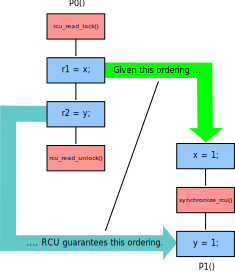
\includegraphics{defer/RCUGuaranteeFwd}}
\caption{RCU Reader and Later Grace Period}
\label{fig:defer:RCU Reader and Later Grace Period}
\end{figure}

The relationship between an RCU read-side critical section and a later
RCU grace period is an if-then relationship, as illustrated by
Figure~\ref{fig:defer:RCU Reader and Later Grace Period}.
If any portion of a given critical section precedes the beginning of
a given grace period, then RCU guarantees that all of that critical
section will precede the end of that grace period.
In the figure, because \co{P0()}'s access to \co{y} precedes
\co{P1()}'s access to this same variable, it is guaranteed that
\co{P0()}'s access to \co{x} will precede \co{P1()}'s access.
In this case, if \co{y}'s final value is 2, then \co{x}'s
final value is guaranteed to also be 2.

\QuickQuiz{}
	What other final values of \co{x} and \co{y} are possible in
	Figure~\ref{fig:defer:RCU Reader and Later Grace Period}?
\QuickQuizAnswer{
	The \co{x == 2 && y == 2} possibility was called out in the text.
	Given that \co{y == 2} implies \co{x == 2}, we know that
	\co{x == 1 && y == 2} is forbidden.
	The following discussion will show that both
	\co{x == 1 && y == 1} and \co{x == 2 && y == 1} are possible.
} \QuickQuizEnd

\begin{figure}[tb]
\centering
\resizebox{3in}{!}{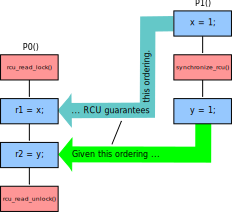
\includegraphics{defer/RCUGuaranteeRev}}
\caption{RCU Reader and Earlier Grace Period}
\label{fig:defer:RCU Reader and Earlier Grace Period}
\end{figure}

The relationship between an RCU read-side critical section and an earlier
RCU grace period is also an if-then relationship, as illustrated by
Figure~\ref{fig:defer:RCU Reader and Earlier Grace Period}.
If any portion of a given critical section follows the end of
a given grace period, then RCU guarantees that all of that critical
section will follow the beginning of that grace period.
In the figure, because \co{P0()}'s access to \co{x} follows
\co{P1()}'s access to this same variable, it is guaranteed that
\co{P0()}'s access to \co{y} will precede \co{P1()}'s access.
In this case, if \co{x}'s final value is 1, then \co{y}'s
final value is guaranteed to also be 1.

\begin{figure}[tb]
\centering
\resizebox{3in}{!}{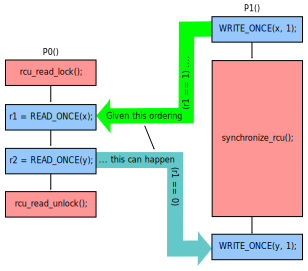
\includegraphics{defer/RCUGuaranteeMid}}
\caption{RCU Reader Within Grace Period}
\label{fig:defer:RCU Reader Within Grace Period}
\end{figure}

Finally, as shown in
Figure~\ref{fig:defer:RCU Reader Within Grace Period},
an RCU read-side critical section can be completely overlapped by
an RCU grace period.
In this case, \co{x}'s final value is 1 and \co{y}'s final value is 2.

However, it cannot be the case that \co{x}'s final value is 2 and \co{y}'s
final value is 1.
This would mean that an RCU read-side critical section had completely
overlapped a grace period, which is forbidden.
RCU's wait-for-readers guarantee therefore has two parts:
(1)~If any part of a given RCU read-side critical section precedes
the beginning of a given grace period, then the entirety of that
critical section precedes the end of that grace period.
(2)~If any part of a given RCU read-side critical section follows
the end of a given grace period, then the entirety of that
critical section follows the beginning of that grace period.
This definition is sufficient for almost all RCU-based algorithms, but
for those wanting more,
simple executable formal models of RCU are available
as part of Linux kernel v4.17 and later, as discussed in
Section~\ref{sec:formal:Axiomatic Approaches and RCU}.
In addition, RCU's ordering properties are examined in much
greater detail in Section~\ref{sec:memorder:RCU}.

Although RCU's wait-for-readers capability really is sometimes used to
order the assignment of values to variables as shown in
Figures~\ref{fig:defer:RCU Reader and Later Grace Period}-\ref{fig:defer:RCU Reader Within Grace Period},
it is more frequently used to safely free data elements removed from
a linked structure, as was done in
Section~\ref{sec:defer:Introduction to RCU}.
The general process is illustrated by the following pseudocode:

\begin{enumerate}
\item	Make a change, for example, remove an element from a linked list.
\item	Wait for all pre-existing RCU read-side critical sections to
	completely finish (for example, by using
	\co{synchronize_rcu()}).
\item	Clean up, for example, free the element that was replaced above.
\end{enumerate}

Given that RCU readers can make forward progress while this update
is in progress, different readers might disagree about the state
of the data structure, a topic taken up by the next section.

\subsubsection{Maintain Multiple Versions of Recently Updated Objects}
\label{sec:defer:Maintain Multiple Versions of Recently Updated Objects}

This section demonstrates how RCU maintains multiple versions of
lists to accommodate synchronization-free readers.

% @@@ \ref{lst:defer:Insertion and Deletion With Concurrent Readers}
%	Describe quick alternating ins_route() and del_route() with
%	concurrent access_route().  Note series of values and total order.
% @@@ Routing as case where reordering is OK.  (Check for repetition.)
% @@@ Isolated lookups as case where software cannot see reordering. (Ditto.)

@@@
Two examples are presented showing how an element
that might be referenced by a given reader must remain intact
while that reader remains in its RCU read-side critical section.
The first example demonstrates deletion of a list element,
and the second example demonstrates replacement of an element.

\paragraph{Example 1: Maintaining Multiple Versions During Deletion}
\label{sec:defer:Example 1: Maintaining Multiple Versions During Deletion}

We can now revisit the deletion example from
Section~\ref{sec:defer:Introduction to RCU},
but now with the benefit of a firm understanding of the fundamental
concepts underlying RCU.
% @@@ \begin{lineref}[ln:defer:Canonical RCU Replacement Example]
% @@@ To begin this new version of the deletion example,
% @@@ we will modify
% @@@ lines~\lnref{search}-\lnref{kfree} in
% @@@ Listing~\ref{lst:defer:Canonical RCU Replacement Example}
% @@@ to read as follows:
% @@@ \end{lineref}

\begin{linelabel}[ln:defer:RCU Deletion From Linked List]
\begin{VerbatimN}[samepage=true,commandchars=\\\[\]]
p = search(head, key);
if (p != NULL) {
	list_del_rcu(&p->list);		\lnlbl[del_rcu]
	synchronize_rcu();		\lnlbl[sync_rcu]
	kfree(p);
}
\end{VerbatimN}
\end{linelabel}

\begin{figure}[tb]
\centering
\resizebox{3in}{!}{\includegraphics{defer/RCUDeletion}}
\caption{RCU Deletion From Linked List}
\label{fig:defer:RCU Deletion From Linked List}
\end{figure}

This code will update the list as shown in
Figure~\ref{fig:defer:RCU Deletion From Linked List}.
The triples in each element represent the values of fields \co{a},
\co{b}, and \co{c}, respectively.
The red-shaded elements
indicate that RCU readers might be holding references to them,
so in the initial state at the top of the diagram, all elements
are shaded red.
Please note that
we have omitted the backwards pointers and the link from the tail
of the list to the head for clarity.

\begin{lineref}[ln:defer:RCU Deletion From Linked List]
After the \co{list_del_rcu()} on
line~\lnref{del_rcu} has completed, the \co{5,6,7}~element
has been removed from the list, as shown in the second row of
Figure~\ref{fig:defer:RCU Deletion From Linked List}.
Since readers do not synchronize directly with updaters,
readers might be concurrently scanning this list.
These concurrent readers might or might not see the newly removed element,
depending on timing.
However, readers that were delayed (e.g., due to interrupts, ECC memory
errors, or, in \co{CONFIG_PREEMPT_RT} kernels, preemption)
just after fetching a pointer to the newly removed element might
see the old version of the list for quite some time after the
removal.
Therefore, we now have two versions of the list, one with element
\co{5,6,7} and one without.
The \co{5,6,7}~element in the second row of the figure is now
shaded yellow, indicating
that old readers might still be referencing it, but that new
readers cannot obtain a reference to it.

Please note that readers are not permitted to maintain references to
element~\co{5,6,7} after exiting from their RCU read-side
critical sections.
Therefore,
once the \co{synchronize_rcu()} on
line~\lnref{sync_rcu} completes, so that all pre-existing readers are
guaranteed to have completed,
there can be no more readers referencing this
element, as indicated by its green shading on the third row of
Figure~\ref{fig:defer:RCU Deletion From Linked List}.
We are thus back to a single version of the list.
\end{lineref}

At this point, the \co{5,6,7}~element may safely be
freed, as shown on the final row of
Figure~\ref{fig:defer:RCU Deletion From Linked List}.
At this point, we have completed the deletion of
element~\co{5,6,7}.
The following example covers replacement.

\paragraph{Example 2: Maintaining Multiple Versions During Replacement}
\label{sec:defer:Example 2: Maintaining Multiple Versions During Replacement}

To start the replacement example,
here are the last few lines of the
example shown in
% @@@ Listing~\ref{lst:defer:Canonical RCU Replacement Example}:

\begin{linelabel}[ln:defer:Canonical RCU Replacement Example (2nd)]
\begin{VerbatimN}[samepage=true,commandchars=\\\[\],firstnumber=15]
q = kmalloc(sizeof(*p), GFP_KERNEL);	\lnlbl[kmalloc]
*q = *p;				\lnlbl[copy]
q->b = 2;				\lnlbl[update1]
q->c = 3;				\lnlbl[update2]
list_replace_rcu(&p->list, &q->list);	\lnlbl[replace]
synchronize_rcu();			\lnlbl[sync_rcu]
kfree(p);				\lnlbl[kfree]
\end{VerbatimN}
\end{linelabel}

\begin{figure}[tbp]
\centering
\resizebox{2.7in}{!}{\includegraphics{defer/RCUReplacement}}
\caption{RCU Replacement in Linked List}
\label{fig:defer:RCU Replacement in Linked List}
\end{figure}

The initial state of the list, including the pointer \co{p},
is the same as for the deletion example, as shown on the
first row of
Figure~\ref{fig:defer:RCU Replacement in Linked List}.

As before,
the triples in each element represent the values of fields \co{a},
\co{b}, and \co{c}, respectively.
The red-shaded elements might be referenced by readers,
and because readers do not synchronize directly with updaters,
readers might run concurrently with this entire replacement process.
Please note that
we again omit the backwards pointers and the link from the tail
of the list to the head for clarity.

The following text describes how to replace the \co{5,6,7} element
with \co{5,2,3} in such a way that any given reader sees one of these
two values.

\begin{lineref}[ln:defer:Canonical RCU Replacement Example (2nd)]
Line~\lnref{kmalloc} \co{kmalloc()}s a replacement element, as follows,
resulting in the state as shown in the second row of
Figure~\ref{fig:defer:RCU Replacement in Linked List}.
At this point, no reader can hold a reference to the newly allocated
element (as indicated by its green shading), and it is uninitialized
(as indicated by the question marks).

Line~\lnref{copy} copies the old element to the new one, resulting in the
state as shown in the third row of
Figure~\ref{fig:defer:RCU Replacement in Linked List}.
The newly allocated element still cannot be referenced by readers, but
it is now initialized.

Line~\lnref{update1} updates \co{q->b} to the value ``2'', and
line~\lnref{update2} updates \co{q->c} to the value ``3'',
as shown on the fourth row of
Figure~\ref{fig:defer:RCU Replacement in Linked List}.

Now, line~\lnref{replace} does the replacement, so that the new element is
finally visible to readers, and hence is shaded red, as shown on
the fifth row of
Figure~\ref{fig:defer:RCU Replacement in Linked List}.
At this point, as shown below, we have two versions of the list.
Pre-existing readers might see the \co{5,6,7} element (which is
therefore now shaded yellow), but
new readers will instead see the \co{5,2,3} element.
But any given reader is guaranteed to see some well-defined list.

After the \co{synchronize_rcu()} on line~\lnref{sync_rcu} returns,
a grace period will have elapsed, and so all reads that started before the
\co{list_replace_rcu()} will have completed.
In particular, any readers that might have been holding references
to the \co{5,6,7} element are guaranteed to have exited
their RCU read-side critical sections, and are thus prohibited from
continuing to hold a reference.
Therefore, there can no longer be any readers holding references
to the old element, as indicated its green shading in the sixth row of
Figure~\ref{fig:defer:RCU Replacement in Linked List}.
As far as the readers are concerned, we are back to having a single version
of the list, but with the new element in place of the old.

After the \co{kfree()} on line~\lnref{kfree} completes, the list will
appear as shown on the final row of
Figure~\ref{fig:defer:RCU Replacement in Linked List}.
\end{lineref}

Despite the fact that RCU was named after the replacement case,
the vast majority of RCU usage within the Linux kernel relies on
the simple deletion case shown in
Section~\ref{sec:defer:Maintain Multiple Versions of Recently Updated Objects}.

\paragraph{Discussion}
\label{sec:defer:Discussion}

These examples assumed that a mutex was held across the entire
update operation, which would mean that there could be at most two
versions of the list active at a given time.

\QuickQuiz{}
	How would you modify the deletion example to permit more than two
	versions of the list to be active?
\QuickQuizAnswer{
	One way of accomplishing this is as shown in
	Listing~\ref{lst:defer:Concurrent RCU Deletion}.

\begin{listing}[htbp]
\begin{VerbatimL}
spin_lock(&mylock);
p = search(head, key);
if (p == NULL)
	spin_unlock(&mylock);
else {
	list_del_rcu(&p->list);
	spin_unlock(&mylock);
	synchronize_rcu();
	kfree(p);
}
\end{VerbatimL}
\caption{Concurrent RCU Deletion}
\label{lst:defer:Concurrent RCU Deletion}
\end{listing}

	Note that this means that multiple concurrent deletions might be
	waiting in \co{synchronize_rcu()}.
} \QuickQuizEnd

\QuickQuiz{}
	How many RCU versions of a given list can be
	active at any given time?
\QuickQuizAnswer{
	That depends on the synchronization design.
	If a semaphore protecting the update is held across the grace period,
	then there can be at most two versions, the old and the new.

	However, suppose that only the search, the update, and the
	\co{list_replace_rcu()} were protected by a lock, so that
	the \co{synchronize_rcu()} was outside of that lock, similar
	to the code shown in
	Listing~\ref{lst:defer:Concurrent RCU Deletion}.
	Suppose further that a large number of threads undertook an
	RCU replacement at about the same time, and that readers
	are also constantly traversing the data structure.

	Then the following sequence of events could occur, starting from
	the end state of
	Figure~\ref{fig:defer:RCU Replacement in Linked List}:

	\begin{enumerate}
	\item	Thread~A traverses the list, obtaining a reference to
		the 5,2,3 element.
	\item	Thread~B replaces the 5,2,3 element with a new
		5,2,4 element, then waits for its \co{synchronize_rcu()}
		call to return.
	\item	Thread~C traverses the list, obtaining a reference to
		the 5,2,4 element.
	\item	Thread~D replaces the 5,2,4 element with a new
		5,2,5 element, then waits for its \co{synchronize_rcu()}
		call to return.
	\item	Thread~E traverses the list, obtaining a reference to
		the 5,2,5 element.
	\item	Thread~F replaces the 5,2,5 element with a new
		5,2,6 element, then waits for its \co{synchronize_rcu()}
		call to return.
	\item	Thread~G traverses the list, obtaining a reference to
		the 5,2,6 element.
	\item	And the previous two steps repeat quickly, so that all
		of them happen before any of the \co{synchronize_rcu()}
		calls return.
	\end{enumerate}

	Thus, there can be an arbitrary number of versions active,
	limited only by memory and by how many updates could be completed
	within a grace period.
	But please note that data structures that are updated so frequently
	probably are not good candidates for RCU.
	That said, RCU can handle high update rates when necessary.
} \QuickQuizEnd

This sequence of events shows how RCU updates use multiple versions
to safely carry out changes in presence of concurrent readers.
Of course, some algorithms cannot gracefully handle multiple versions.
There are techniques
for adapting such algorithms to RCU~\cite{PaulEdwardMcKenneyPhD},
but these are beyond the scope of this section.

\subsubsection{Summary of RCU Fundamentals}
\label{sec:defer:Summary of RCU Fundamentals}

This section has described the three fundamental components of RCU-based
algorithms:

\begin{enumerate}
\item	a publish-subscribe mechanism for adding new data,

\item	a way of waiting for pre-existing RCU readers to finish,\footnote{
		This component is described in much greater detail in
		Section~\ref{sec:memorder:RCU}.}
	and

\item	a discipline of maintaining multiple versions to permit
	change without harming or unduly delaying concurrent RCU readers.
\end{enumerate}

\QuickQuiz{}
	How can RCU updaters possibly delay RCU readers, given that the
	\co{rcu_read_lock()} and \co{rcu_read_unlock()}
	primitives neither spin nor block?
\QuickQuizAnswer{
	The modifications undertaken by a given RCU updater will cause the
	corresponding CPU to invalidate cache lines containing the data,
	forcing the CPUs running concurrent RCU readers to incur expensive
	cache misses.
	(Can you design an algorithm that changes a data structure
	\emph{without}
	inflicting expensive cache misses on concurrent readers?
	On subsequent readers?)
} \QuickQuizEnd

These three RCU components
allow data to be updated in face of concurrent readers, and
can be combined in different ways to
implement a surprising variety of different types of RCU-based algorithms.
However, it is usually better to work at higher levels of abstraction.
To this end, the next section describes the Linux-kernel API, which
includes simple data structures such as lists.
